\documentclass[12pt,a4paper]{article}
\usepackage{graphicx, color}
\usepackage[margin=2cm]{geometry}
\usepackage{multirow}
\usepackage{sectsty}
\usepackage{amssymb}
\usepackage{wrapfig}
\usepackage{natbib}
\usepackage{hyperref}
%\usepackage{url}
%\usepackage[pdftex]{graphicx}

\sectionfont{
%	\sectionrule{0pt}{0pt}{-5pt}{1pt}
}
\begin{document}
\title{\color{red} GPROF Report}
\maketitle

\begin{table}[ph]
\large
\centering
\begin{tabular}{c c c}
\hline
GroupName &RollNumber &Name\\
\hline 
\multirow{3}{*}{!JustCoders} &140050031 &C Vishwesh\\ &140070003 &Saurabh Garg\\&140070031 &Aviral Kumar\\
\hline
\end{tabular}
\end{table}
\pagebreak

\section*{Observations :}

The first call graph that was obtained before optimizing manually and when make file was generated in Debug mode :
\begin{figure}[ht!]
\centering
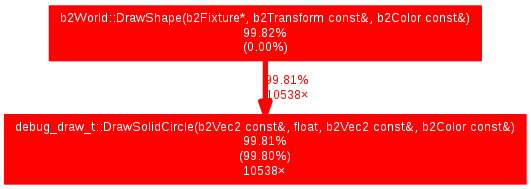
\includegraphics[scale=0.75]{./debugVersion_before.png}
\caption{Call Graph}
\end{figure} 

The simulation was very slow its speed was decreased drastically due a change in render.cpp file. There was a extra loop added in render.cpp file that was taking too much of run time but was of no use. 
\\

To get rid of this i.e. to make simulation fast there was an optimazation needed in render.cpp file so we commented out that line and then rebuilded the box2d simulation.
This time simulation was at normal speed  and call graph generated looked like :
\begin{figure}[ht!]
\centering
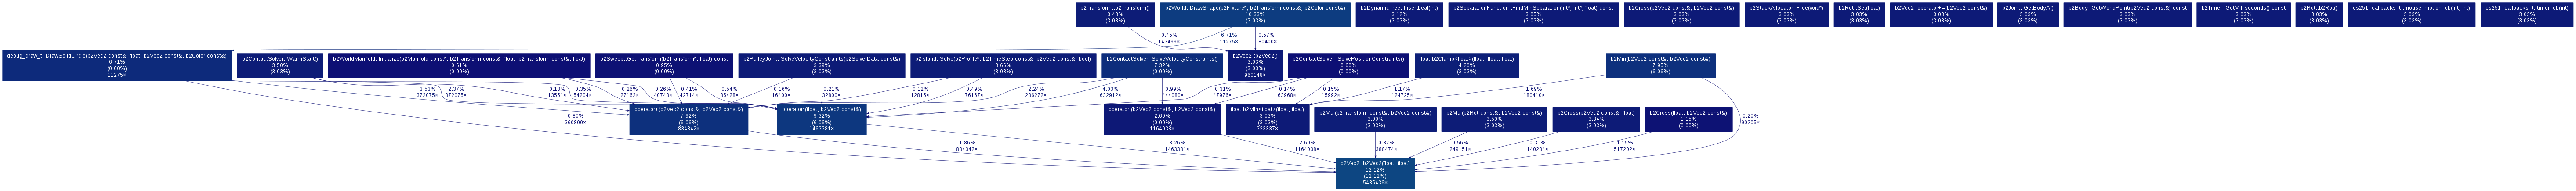
\includegraphics[scale=0.08]{./debugVersion_after.png}
\caption{Call Graph}
\end{figure} 
\\(Graph is not legible in this so we have submitted png file)
\\
On recompiling the code after setting the release mode and adding -O3 in CPPCOMPILER flag graph looked like :
\begin{figure}[ht!]
\centering
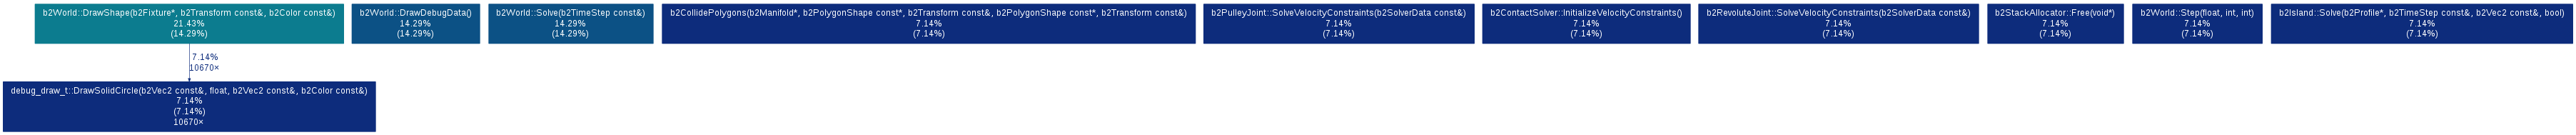
\includegraphics[scale=0.2]{./releaseVersion.png}
\caption{Call Graph}
\end{figure} 
\\	
In this we removed -g flag because -g flag tells the compiler to generate debugging information. It has no impact on whether or not a core file will be generated.
This time also speed of simulation was normal.
\pagebreak
\section*{Profile Data:}

First five profile functions in initial debug mode without manual optimization : 
\begin{verbatim}
1. debug_draw_t::DrawSolidCircle(b2Vec2 const&, float, b2Vec2 const&, b2Color const&)
2. b2Vec2::b2Vec2(float, float)
3. b2ContactSolver::SolvePositionConstraints()
4. operator*(b2Vec2 const&, b2Vec2 const&)
5. operator-(b2Vec2 const&, b2Vec2 const&)
\end{verbatim}
First five profile functions in initial debug mode with manual optimization :
\begin{verbatim}
1. b2Vec2::b2Vec2(float, float)
2. operator*(float, b2Vec2 const&)
3. operator+(b2Vec2 const&, b2Vec2 const&)
4.  b2Min(b2Vec2 const&, b2Vec2 const&)
5. b2Vec2::b2Vec2()
\end{verbatim}
First five profile functions in release mode with -O3 flag optimization :
\begin{verbatim}
1. b2World::DrawDebugData()
2. b2World::Solve(b2TimeStep const&)
3. b2World::DrawShape(b2Fixture*, b2Transform const&, b2Color const&)
4. debug_draw_t::DrawSolidCircle(b2Vec2 const&, float, b2Vec2 const&, b2Color const&)
5.  b2CollidePolygons(b2Manifold*, b2PolygonShape const*, b2Transform const&, 
b2PolygonShape const*, b2Transform const&) 
\end{verbatim}
But actually everytime on execution of simulation the order of functions in the profile data changes as for some functions time difference is of very small order
\\ 
\\
\textbf{Interesting Observation : }
The contact solver function is mostly at the top in all the profiles and each time on compilation we have different functions at top in profile data in debug release mode .
\end{document}

